%
% kapazitaet.tex
%
% (c) 2020 Prof Dr Andreas Müller, Hochschule Rapperswil
%
\begin{frame}
\frametitle{Infektion bis zur Kapazitätsgrenze}
\begin{columns}[t]
\begin{column}{0.48\hsize}
\begin{block}{Strategie}
\begin{enumerate}
\item<2-> Sobald $I=I_0$ Lockdown derart, dass $I=\text{const}$
\item<7-> $S$ klein genug: ``Let it rip'' (Herdenimmunität)
\end{enumerate}
\end{block}
\uncover<3->{
\begin{block}{Lockdown-Massnahmen}
So, dass $\dot{I}=0$, also
\begin{align*}
0
=
\frac{dI}{dt}
&=
\beta S I - \gamma I
=
(\beta S - \gamma) I
\\
\uncover<4->{\Rightarrow \beta}&\uncover<4->{= \frac{\gamma}{S}}
\end{align*}
\end{block}}
\end{column}
\begin{column}{0.48\hsize}
\uncover<5->{
\begin{block}{Wie hängt $\beta$ von $S$ ab?}
\begin{center}
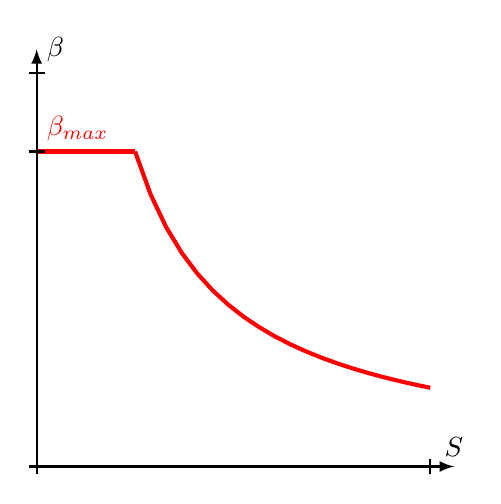
\begin{tikzpicture}[>=latex,thick]
\def\betamax{0.8}
\def\gammavalue{0.2}
\pgfmathparse{\gammavalue/\betamax}
\xdef\Sthreshold{\pgfmathresult}
\uncover<6->{
	\draw[color=red,line width=1.5pt] plot[domain=\Sthreshold:1,samples=20]
		({5*\x},{5*\gammavalue/\x});
}
\uncover<8->{
	\draw[color=red,line width=1.5pt]
		(0,{5*\betamax})--({5*\Sthreshold},{5*\betamax});
	\node[color=red] at (0,{5*\betamax}) [above right]
		{$\beta_{\text{max}}$};
	\draw (-0.1,{5*\betamax})--(0.1,{5*\betamax});
}
\draw (5,-0.1)--(5,0.1);
\draw (-0.1,5)--(0.1,5);
\draw[->] (-0.1,0)--(5.3,0) coordinate[label={$S$}];
\draw[->] (0,-0.1)--(0,5.3) coordinate[label={right:$\beta$}];
\end{tikzpicture}
\end{center}
\end{block}}
\end{column}
\end{columns}
\end{frame}
